\documentclass[11pt]{article}
\usepackage[utf8]{inputenc}
\usepackage[T1]{fontenc}
\usepackage{lmodern}
\usepackage{geometry}
\usepackage{tikz}
\usetikzlibrary{arrows.meta,shapes.geometric}

\geometry{paperwidth=16cm,paperheight=6.4cm,margin=0cm}
\pagestyle{empty}
\setlength{\parindent}{0pt}

\definecolor{ctxFill}{RGB}{238,242,245}
\definecolor{ctxLine}{RGB}{155,168,179}
\definecolor{ctxText}{RGB}{38,52,67}
\definecolor{exFill}{RGB}{220,233,247}
\definecolor{exLine}{RGB}{23,54,93}
\definecolor{prFill}{RGB}{200,240,236}
\definecolor{prLine}{RGB}{8,127,140}
\definecolor{prText}{RGB}{6,79,87}

\begin{document}
\noindent
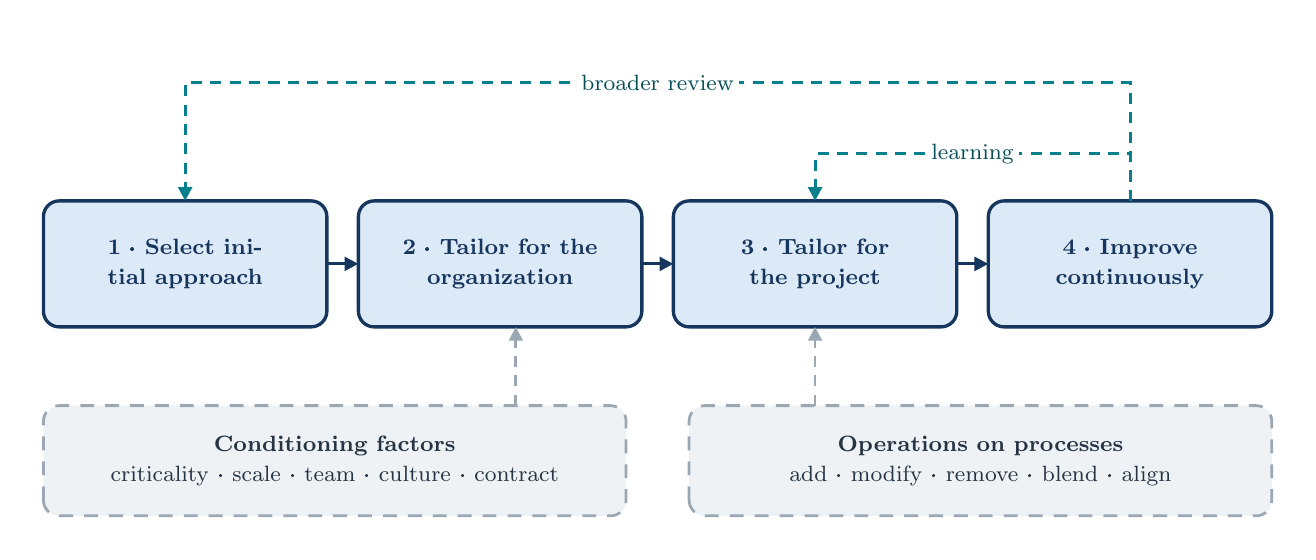
\begin{tikzpicture}[x=1cm,y=1cm,font=\small]
  \path[use as bounding box] (0,0) rectangle (16,6.4);
  \draw[fill=exFill,draw=exLine,line width=1.2pt,rounded corners=0.2cm] (0.2,2.6) rectangle (3.8000000000000003,4.2);
  \node[align=center,text width=3.3cm,text=exLine] at (2.0,3.4) {\footnotesize\textbf{1 · Select initial approach}};
  \draw[draw=exLine,line width=1.1pt,-{Triangle[length=5pt,width=5pt]}] (3.8000000000000003,3.4) -- (4.2,3.4);
  \draw[fill=exFill,draw=exLine,line width=1.2pt,rounded corners=0.2cm] (4.2,2.6) rectangle (7.800000000000001,4.2);
  \node[align=center,text width=3.3cm,text=exLine] at (6.0,3.4) {\footnotesize\textbf{2 · Tailor for the organization}};
  \draw[draw=exLine,line width=1.1pt,-{Triangle[length=5pt,width=5pt]}] (7.800000000000001,3.4) -- (8.2,3.4);
  \draw[fill=exFill,draw=exLine,line width=1.2pt,rounded corners=0.2cm] (8.2,2.6) rectangle (11.799999999999999,4.2);
  \node[align=center,text width=3.3cm,text=exLine] at (10.0,3.4) {\footnotesize\textbf{3 · Tailor for the project}};
  \draw[draw=exLine,line width=1.1pt,-{Triangle[length=5pt,width=5pt]}] (11.799999999999999,3.4) -- (12.2,3.4);
  \draw[fill=exFill,draw=exLine,line width=1.2pt,rounded corners=0.2cm] (12.2,2.6) rectangle (15.799999999999999,4.2);
  \node[align=center,text width=3.3cm,text=exLine] at (14.0,3.4) {\footnotesize\textbf{4 · Improve continuously}};
  \draw[draw=prLine,line width=1.1pt,dash pattern=on 4pt off 3pt,-{Triangle[length=5pt,width=5pt]}] (14.0,4.2) -- (14.0,4.8) -- (10.0,4.8) -- (10.0,4.2);
  \node[text=prText,fill=white,inner sep=2pt] at (12.0,4.8) {\footnotesize learning};
  \draw[draw=prLine,line width=1.1pt,dash pattern=on 4pt off 3pt,-{Triangle[length=5pt,width=5pt]}] (14.0,4.2) -- (14.0,5.7) -- (2.0,5.7) -- (2.0,4.2);
  \node[text=prText,fill=white,inner sep=2pt] at (8.0,5.7) {\footnotesize broader review};
  \draw[fill=ctxFill,draw=ctxLine,line width=1pt,dash pattern=on 5pt off 4pt,rounded corners=0.2cm] (0.2,0.2) rectangle (7.6,1.6);
  \node[align=center,text=ctxText,text width=7.0cm] at (3.9,0.9) {\footnotesize\textbf{Conditioning factors}\\ criticality · scale · team · culture · contract};
  \draw[draw=ctxLine,line width=1pt,dash pattern=on 4pt off 3pt,-{Triangle[length=5pt,width=5pt]}] (6.2,1.6) -- (6.2,2.6);
  \draw[fill=ctxFill,draw=ctxLine,line width=1pt,dash pattern=on 5pt off 4pt,rounded corners=0.2cm] (8.4,0.2) rectangle (15.8,1.6);
  \node[align=center,text=ctxText,text width=7.0cm] at (12.1,0.9) {\footnotesize\textbf{Operations on processes}\\ add · modify · remove · blend · align};
  \draw[draw=ctxLine,line width=1pt,dash pattern=on 4pt off 3pt,-{Triangle[length=5pt,width=5pt]}] (10.0,1.6) -- (10.0,2.6);
\end{tikzpicture}
\end{document}
